\documentclass[../main/main.tex]{subfiles}


\begin{document}

\section{March 28th, 2019}
\subsection{Bipartite Matching}
\begin{figure}[h!]
	\centering
	
\includegraphics[width=0.4\textwidth]{3-28-bipartite-graph}
	\caption{Example of Bipartite Graph}
	\label{fig:3-28-bipartitegraph}
\end{figure}
\begin{definition}\index{bipartite graph}
	A \vocab{bipartite graph} is a graph with a bipartition, with all edges only crossing the bipartition.
\end{definition}
\begin{itemize}
	\item An edge represents a person willing to do a job
	\item Each person can be assigned to at most one job
	\item Each job can be occupied by at most one person
	\item QUESTION: is it possible to assign the employees such that every employee gets one job and each job is filled? 
\end{itemize}
\begin{remark}\index{maximal matching} \index{maximum matching}
	A \vocab{maximal matching} is a matching for which if you add another edge, it would not be a matching. A \vocab{maximum matching} is the matching with maximum cardinality. A maximum matching is always a maximal, but a maximal is not always a maximum.
\end{remark}
\begin{definition}\index{neighborhood}
	A \vocab{neighborhood} of a subset of vertices, $A$, is all the vertices they are connected to a vertex in $A$ by an edge in $E$. e.g. \[
		N\left( \{A,B,D\}  \right) =\{q,s\} 
	.\] 
\end{definition}
\begin{remark}
	The following are necessary conditions to have a perfect matching:
	\begin{itemize}
		\item The size of each side in this partition is the same.
		\item The size of the neighborhood of any subset is greater than or equal to the size of the subset. e.g. in the example above \[
				|N(S)|\ge |S|,\ \forall S \subseteq L
		.\] 
	\end{itemize}
	\vspace{-0.2cm}
	These will be proven to be sufficient later 
\end{remark}\vspace{-0.2cm}
From weak duality, we have that for any graph, the size of the max matching is less than or equal to the size of the min vertex cover.
\vspace{-0.45cm}
\subsection{Bipartite Matching as a Max Flow Problem}
\begin{figure}[h!]
	\centering
	
\includegraphics[width=0.5\textwidth]{3-28-bipartite-flow}
	\caption{Matching as a Max Flow Problem (all $c(s,v)$ and  $c(t,v)$ is 1)}
	\label{fig:3-28-bipartiteflow}
\end{figure}\vspace{-0.4cm}
Easy observations:
\begin{enumerate}
	\item Suppose you have an integral flow of value $k$ in $G'$, the flow network. Then you have a matching of size $k$ in $G$.
	\item Suppose you have a matching os size $k$ is $G$. Then you have a flow of value $k$.
\end{enumerate}
\begin{algo}
We can  solve the problem of finding a max matching in a bipartite graph in polynomial time by reducing it to max flow as follows:
	\begin{itemize}
		\item Let $L,R$ denote the vertices on the left and right side of the bipartite graph respectively. Direct edges of the graph from left to right.
		\item Add 2 new nodes $s$ and  $t$, and add direct edges from  $s$ to all vertices in  $L$  and from all vertices in $R$ to  $t$.
		\item Set $c(s,v) =c(v,t)=1$ and $\infty$ for edges from $L$ to $R$.
		\item Find the max flow in the network, assuming that the flow is integral.
		\item Return the edges of the graph in which flow is $1$.
	\end{itemize}
	This algorithm outputs a maximum matching.
\end{algo}
	\begin{proof}
		Follows from (1) and (2)
	\end{proof}

\begin{remark}
	Note that we can use any FF method, since the number of iteration is bounded by $|V|$. Since each iteration takes  $O(|E|)$ time, we have a $O(|V| E|)$ algorithm.

We can run the FF method to find the maximum matching, as all capacities are integral values (all edges have capacity 1). If we have a flow, we will have a matching equal to $|f|$.
	\end{remark}
	\begin{remark}
		This algorithm only works for bipartite graphs, but there is another polynomial time algorithm that can find the maximum matching of arbitrary graphs (albeit more complicated).
	\end{remark}
	\subsection{Perfect Matching in Bipartite Graphs}

\begin{definition}\index{perfect matching}
	A \vocab{perfect matching} is a matching which "covers" all the vertices.
\end{definition}
\begin{theorem}[Hall's Theorem]
	A bipartite graph $G(V,E)$ with bipartition $\left( L,R \right) $ has a perfect matching if and only if: 
	\begin{enumerate}
		\item $|L|=|R|$ ; and 
		\item $\forall A\subseteq L$, we have \[
				|A|\le |N(A)|
		.\]  
	\end{enumerate}
	These properties have been shown to be necessary conditions, but they are also sufficient conditions (using max-flow min-cut).
\end{theorem}

\begin{proof}
	Suppose that $G$ does not have a perfect matching and  $|L|=|LR|$. Then we will prove that  $\exists A\subseteq L$ such that $|A|>|N(A)|$, i.e. (2) will be violated. We will use the same reduction to the max-flow problem. Recall the flow network $G'$ as before.
	\begin{figure}[h!]
		\centering
		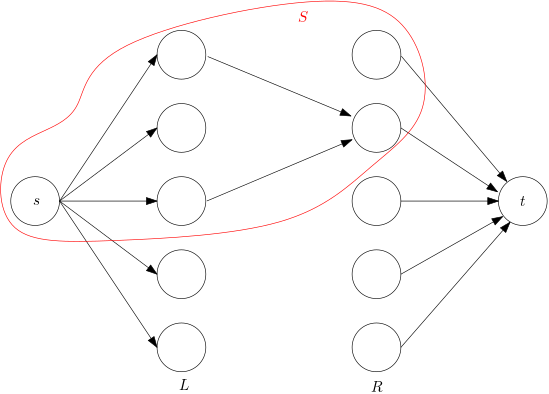
\includegraphics[width=0.45\textwidth]{3-28-bipartite-mincut}
		\caption{Example of a cut $S$}
		\label{fig:}
	\end{figure}

	Consider the $s-t$ cut $S$ of minimum capacity. The capacity of this cut is \[
	|L-S|+|R\cap S|
	.\] 

	Note that there is no edges from $L\cap S$ that goes to $R\cap (V-S)$, since the capacity of the cup would be infinite, which would violate the max flow min cut thoerem, since the max flow is clearly finite. This means that  \[
		N(L\cap S)\subseteq R\cap S
	.\]
	Since $G$ does not have a perfect matching, if we let $|L|=|R|=n$  \[
	\text{Size of max matching}<n \implies \text{Value of max flow }< n\implies \text{Capacity of min cut }<n 
	.\] 
	Note that \[
	|L-S|+|R\cap S|<n=|L-S|+|L\cap S|
	,\] which means \[
	|L\cap S|>|R\cap S| 
	.\]  
\end{proof}


\end{document}

